\subsection{Ontology}
\label{subsec_method_ontology}

As described in the previous section, different data sources with different data formats were used. 
To create a unified dataset and therefore enable simple querying over all data, a unified ontology was defined.


The following resources, defined by the dataset, can mostly be represented by dbpedia entities. 
In most cases a dbpedia entity is available.
If no dbpedia entity was present freebase entities or self defined ones were used.

\begin{itemize}
\item Movie: dbpedia-owl:Film
\item Award: dbpedia-owl:Award
\item MoviePerson: dbpedia-owl:Person
\item Character: freebase:film/performance
\item Aka (also known as): aka
\item ReleaseInfo: releaseInfo

\end{itemize}

A MoviePerson can be beside a dbpedia-owl:Person also another type, depending on the job the person plays. 
As shown in Figure \ref{fig_ontology} a distinction between e.g. director, writer, producer was made.
In Figure \ref{fig_ontology} are also the relations between the listed resources shown.

%dbpedia-owl:Actor,
%dbpedia-owl:director,
%dbpedia-owl:Writer,
%dbpedia-owl:producer,
%dbpedia-owl:coProducer,
%dbpedia-owl:makeUpArtist,
%dbpedia-owl:costumeDesigner,
%dbpedia-owl:specialEffects,
%dbpedia-owl:setDesigner,
%dbpedia-owl:storyEditor


\begin{figure}[h!]
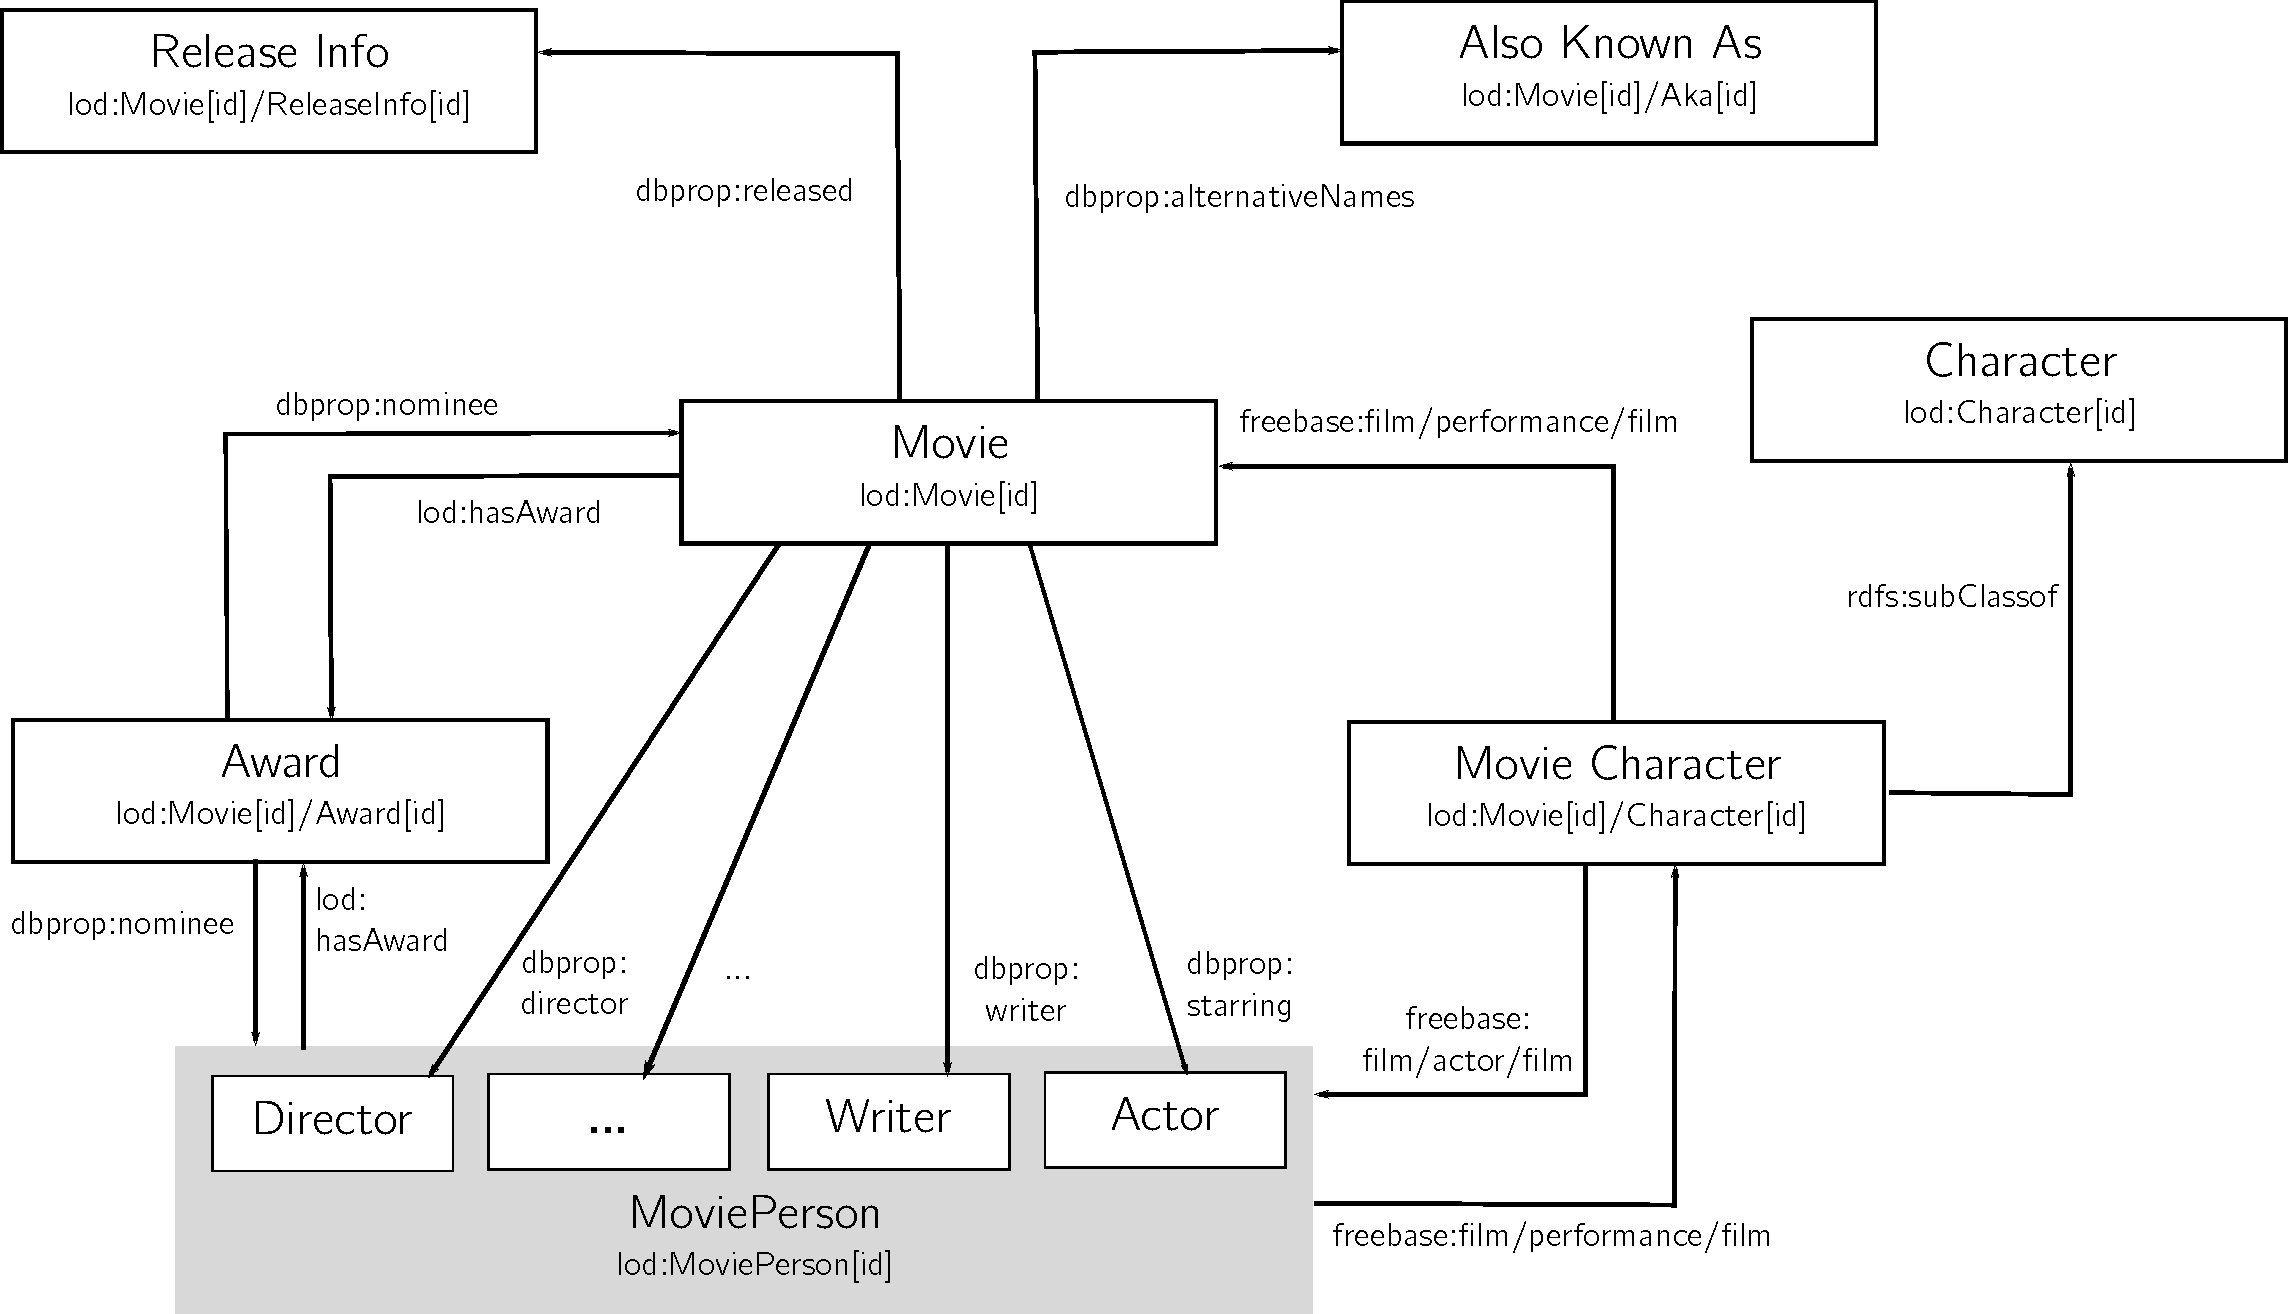
\includegraphics[width=\textwidth]{images/ontology.pdf}
\caption{Ontology}
\label{fig_ontology}
\end{figure}

The character resource must also be treated special. It exists movies which have




%onthology -> movie character (james bond- john connory), classes, picture presentation, dbpedia-props > freebase > own